\documentclass{beamer}
%% macros just for semantics

% ---- Minimal setup (XeLaTeX) ----
\usepackage{fontspec}
\defaultfontfeatures{Ligatures=TeX}
%\usepackage{luatexja}
%\usepackage{luatexja-fontspec}
%\ltjsetparameter{jacharrange={-9}}
\setmainfont{TeX Gyre Pagella}
\setsansfont{TeX Gyre Heros}
\setmonofont{Inconsolata} % TeX Gyre Cursor} %  Fira Mono}
% Auto-switch by Unicode block
\usepackage[CJK,Emoticons,IPAExtensions,SpacingModifierLetters,PhoneticExtensions]{ucharclasses}
\newfontfamily\devanagarifont{Noto Sans Devanagari}
\setTransitionsFor{Devanagari}{\devanagarifont}{\normalfont}
\newfontfamily\jafont{Noto Sans CJK JP}
\newfontfamily\krfont{Noto Sans CJK KR}
\newfontfamily\hanfont{Noto Sans CJK SC} % or TC
\setTransitionsForChinese{\hanfont}{\normalfont}
\setTransitionsForKorean{\krfont}{\normalfont}
\setTransitionsForJapanese{\jafont}{\normalfont}
\pdfstringdefDisableCommands{%
  \def\jafont{}%
  \def\devanagarifont{}%
}
\newcommand{\jpf}[1]{{\jafont #1}}
\newcommand{\ipa}[1]{{\ipafont\selectfont #1}}

\newfontfamily\ipafont{Gentium}  % or DejaVu Sans, Charis SIL, Doulos SIL

\setTransitionsFor{IPAExtensions}{\ipafont}{\normalfont}
\setTransitionsFor{SpacingModifierLetters}{\ipafont}{\normalfont}
\setTransitionsFor{PhoneticExtensions}{\ipafont}{\normalfont}

%\newfontfamily\emojifont{Symbola}
%\setTransitionsFor{Emoticons}{\emojifont}{\normalfont}

%\setTransitionsFor{Han}{\hanfont}{\normalfont}
% \newfontfamily\emoji{Noto Color Emoji}[Renderer=Harfbuzz,Scale=MatchLowercase]
% \newcommand{\e}[1]{{\emoji #1}}

\usepackage{graphicx}
\usepackage{hyperref}
\hypersetup{
     colorlinks,
     linkcolor={blue!50!black},
     citecolor={red!50!black},
     urlcolor={blue!80!black}
   }
\usepackage{booktabs}
\usepackage{microtype}
\usepackage{multicol}

\newcommand{\txx}[1]{\textbf{\textcolor{blue}{#1}}}

% --- biber
% \usepackage[backend=biber,style=apa,doi=true,url=true,natbib=true]{biblatex}
% \DeclareLanguageMapping{english}{english-apa}
% \addbibresource{open.bib}
\usepackage[round]{natbib}

% ---- Beamer look ----
\usetheme{Boadilla}
\usecolortheme{seahorse}
\setbeamertemplate{navigation symbols}{}
\setbeamertemplate{itemize items}[circle]
\setbeamertemplate{itemize subitem}[triangle]
%\setbeamertemplate{footline}[frame number]
\setbeamerfont{block body example}{size=\small}
\setbeamerfont{block title example}{size=\small}  % optional: adjust title too
% ---- Section outline slide ----
\AtBeginSection[]{
  \begin{frame}
    \frametitle{Roadmap}
    \small
    \tableofcontents[currentsection, hideothersubsections]%, hideallsubsections]
  \end{frame}
}
\logo{\includegraphics[width=15mm]{img/UP_logo_FF_horizont_en.png}}

% ---- other packages
\usepackage{tikz}
\usetikzlibrary{positioning}

\usepackage{longtable}

% ---- Linguistics

\usepackage{langsci-gb4e}
\usepackage{langsci-avm}

\usepackage[normalem]{ulem}
\newcommand{\ul}{\uline}
\newcommand{\ull}{\uuline}
\newcommand{\udl}{\dashuline}
\newcommand{\uwl}{\uwave}

\usepackage[e,f,j]{mtg2e}
\newcommand{\cmn}{\mtciteform}
\newcommand{\kor}{\mtciteform}
\newcommand{\cs}{\mtciteform}
\renewcommand{\mtcitestyle}[1]{\textcolor{teal}{\textit{#1}}}
\usepackage{xcolor}
 \newcommand{\bs}{\textbackslash}   % backslash
 \newcommand{\cmd}[1]{{\bf \color{red}#1}}   % highlights command
 \newcommand{\wemp}[1]{\ul{#1}}   % highlight
 \newcommand{\emp}[1]{\textbf{\color{blue}{#1}}}   % highlight
 \newcommand{\rel}[1]{\textsc{\color{blue}{#1}}}
 %%% imi zokusei
 \newcommand{\iz}[1]{\textup{\texttt{\color{blue}{\textbf{#1}}}}}
 \newcommand{\con}{\iz}
 \newcommand{\lnk}[1]{\rel{#1}}
\newcommand{\cmp}[1]{{[\textsc{#1}]}}
\newcommand{\elem}[1]{\ensuremath{\langle}\texttt{#1}\ensuremath{\rangle}}
 \newcommand{\lex}[1]{\textbf{\color{teal}{\textit{#1}}}}
 \newcommand{\lng}[1]{\textcolor{teal}{\textit{#1}}}
\newcommand{\wn}[3]{\lex{#1}\ensuremath{_{#2:#3}}}
\usepackage{relsize,xspace}
\newcommand{\wnida}[1]{\asort{\wnid{#1}}}
\newcommand{\wnid}[1]{\textsf{\smaller #1}}
\newcommand{\into}{\ensuremath{\rightarrow}\xspace}
\newcommand{\ent}{\ensuremath{\Rightarrow}\xspace}
\newcommand{\nent}{\ensuremath{\not\Rightarrow}\xspace}
\newcommand{\tot}{\ensuremath{\leftrightarrow}\xspace}

\newcommand{\MyLogo}[1]{}

% \newcommand{\task}{\marginpar{\raisebox{-2ex}{
%       \hspace{-0.5em}\reflectbox{\includegraphics[width=2em]{img/detective.pdf}}}}}
\newcommand{\task}{\hfill{?}}


\setbeamercolor{taskc}{fg=black,bg=red!10}

\newenvironment{taskb}[1][]{%
  \begin{beamercolorbox}[rounded=true,shadow=true,wd=\linewidth,sep=0.5em]{taskc}
    \ifx\relax#1\relax
      % No title - just show content
    \else
      % Title provided
      \textbf{\large ?} #1
      \par\vspace{0.3em}
    \fi
}{%
  \end{beamercolorbox}
  \vspace{0.5em}
}
%%% Sherlock Holmes
\newcommand{\sh}[1]{\lowercase{\href{https://fcbond.github.io/sh-canon/#1.html}}{#1}}

\date[2026]{DAS \{4|5\}UJ2 2026\\
Slides are open source (CC BY 4.0)}

\author{Francis \textbf{Bond}}
\institute[Palacký]{Department of Asian Studies,
\\  Palacký University, Olomouc, Czechia
\\[1.5ex] \url{<bond@ieee.org>}}

\title[Syntax and Semantics]{Introduction}

\usepackage{forest}


\begin{document}

\maketitle

%\include{schedule}

\section{Welcome}
\begin{frame}{Welcome!}
\begin{itemize}
\item In this course we will introduce you to the study of grammar and meaning
  \begin{itemize}
  \item Syntax
    \begin{itemize}
    \item How words differ from each other
    \item How they can be combined to make larger structures
    \end{itemize}
  \item Semantics and Pragmatics
    \begin{itemize}
    \item How meaning is built up from words and phrases
    \item How meaning depends on context
    \end{itemize}
  \end{itemize}
\item We will ground the analysis with real examples from the Sherlock Holmes stories and the War with the Newts
  \begin{itemize}
  \item I try to make this as enjoyable as possible
  \end{itemize}
\end{itemize}

\end{frame}


\begin{frame}{Overview}
  \begin{itemize}
  \item The course is co-taught by Joanna Ut-Seong Sio (Syntax)
  \item The timetable is available in Moodle.   
  \item Most weeks you will have a lecture and a tutorial
   \\ (no tutorial on the first and last weeks)
  \item Assessment
    \begin{itemize}
    \item Satisfactorily complete ALL tutorial sets (40 marks) and attend 80\% of the tutorials. Students will discuss and complete the problem sets with the tutors during tutorials and hand them in at the next tutorial. 
    \item Do the assigned readings to make sure you understand the content of the course
    \item Two quizzes (60 marks, 30 marks each). Students must obtain 20 marks out of 30 marks for each test to pass the course. 
    \item People doing 5UJ2 get an extra small project (TBA).
    \end{itemize}
  \end{itemize}
\end{frame}


\begin{frame}{Textbook and Readings}

  \begin{itemize}
  \item Syntax: Carnie (2012) \textit{Syntax A Generative Introduction}, 3rd Edition. Wiley-Blackwell.
  \item Semantics: Saeed, John (2015) \textit{Semantics}. 4rd
  Edition. Wiley-Blackwell.
\end{itemize}

\begin{itemize}
\item If you want to know more about semantics I recommend
  \begin{itemize}
  \item Paul Kroeger (2022) \textit{Analyzing meaning: An introduction to semantics and pragmatics}. 3rd edition.  Language Science Press. \href{https://langsci-press.org/catalog/book/359}{DOI: 10.5281}  (Open Source)
%  \item Saeed, John (2015) \textit{Semantics}. 4rd Edition. Wiley-Blackwell. 
  \item Lyons, John (1977) \textit{Semantics}.  Cambridge University Press
  \end{itemize}
\end{itemize}
\end{frame}

\section{Introduction to Semantics}

\begin{frame}{What is Semantics}
\begin{itemize}
\item Very broadly, semantics is the study of meaning
  \begin{itemize}
  \item Word meaning
  \item Sentence meaning
  \item Contextual meaning (pragmatics)
  \end{itemize}
\item Why do we want to study meaning?
  \begin{itemize}
  \item It underlies our understanding of the world
  \item It is fundamental to our thinking, but we don't consciously know what we are doing
  \end{itemize}
\item What kind of knowledge does it take for a speaker to produce language and for a hearer to comprehend language? 
\end{itemize}

\end{frame}



\begin{frame}{Layers of Linguistic Analysis}
\begin{enumerate}\addtolength{\itemsep}{-0.75ex}
\item Phonetics \& Phonology
\item Morphology
\item Syntax
\item \txx{Semantics}
\item Pragmatics
\item Stylistics
\end{enumerate}
% Two theories
% \begin{itemize}
% \item Semantics is \txx{autonomous}, a separate module
% \item Semantics is \txx{integrated} with other knowledge, inseparable
%   \begin{itemize}
%   \item linguistic knowledge is inseparable from encyclopedic knowledge
%   \end{itemize}
% \end{itemize}
\end{frame}

\begin{frame}[allowframebreaks]{Do people share a common conceptual system?}

\begin{itemize}
\item What is a \lex{high school}?
\item What color is \lex{blue}?
\item What does \lex{verb} mean?
\item What is  \lex{carrot cake}?
\item What color are \lex{traffic lights}?
\end{itemize}

\framebreak

\begin{quotation}
  
Japanese traffic lights are green (as required by international
agreements).  However they are typically called 青い \jpn[blue]{aoi},
the same word as the color of the sky.  Historically this color
historically covered both green and blue ``grue'',
with 緑 \jpn[green]{midori} being a later addition.  For this reason,
the Japanese government decided in 1973 to change the color of the go
light to the bluest possible hue of green!


\hfill \href{https://www.japantimes.co.jp/life/2013/02/25/language/the-japanese-traffic-light-blues-stop-on-red-go-on-what/}{The Japanese traffic light blues: Stop on red, go on what?}
\end{quotation} 
\end{frame}

\begin{frame}{Word Meaning and Sentence Meaning}

\begin{itemize}
\item We store information about words in our \txx{mental lexicon}
  \begin{itemize}
  \item It is still unclear what exactly a word is!
  \end{itemize}
\item Words can be combined to form an infinite number of expressions
  \begin{itemize}
  \item This building up of meaning is referred to as \txx{composition}
  \item If the meaning of the whole can be deduced from the parts then it is \txx{compositional}
  \end{itemize}
\end{itemize}
\end{frame}

\begin{frame}{Reference and Sense}

\begin{itemize}
\item Words \txx{refer} to things in the world (like \iz{unicorn}s)
\item The meaning of a word across different contexts is often referred to as its \txx{sense}
  \begin{itemize}
  \item Same word can refer to different things
    \begin{itemize}
    \item English: \eng{I put my money in the \ul{bank}}
    \item English: \eng{I fell asleep at the river \ul{bank}}
    \end{itemize}
  \item Same basic concept can have different boundaries
    \begin{itemize}
    \item French: \eng[sheep/mutton]{mouton}
    \item English: \eng{sheep} vs \eng{mutton}
      
    \item Japanese: \eng[dove/pigeon]{hato}
    \item English: \eng{dove} vs \eng{pigeon}
    \end{itemize}
  \end{itemize}
\end{itemize}



\end{frame}

\begin{frame}{Representing meaning}
\MyLogo{Also vector space, description, images, video, \ldots}
\begin{itemize}
\item One of our goals will be to represent meaning
\item There are various ways to do this
  \begin{itemize}
  \item Syntactic trees
  \item Logical forms
  \item Thesauri and Ontologies 
  \item Translation
  \item Paraphrasing
  \end{itemize}
Can you think of others?

\item At the end of this course you should be able to use these to
  describe many aspects of word meaning
\end{itemize}


\end{frame}



\begin{frame}{Further Reading}

\begin{itemize}
\item Introduction What does it mean to mean?
  \begin{itemize}
  \item Saeed: \S~1
  \end{itemize}
\end{itemize}
\end{frame}

%\subsection{Self  Introduction}

\begin{frame}[allowframebreaks]{Self Introduction}

\begin{itemize}
%\item Francis Bond 
\item BA in Japanese and Mathematics 
  \hfil\raisebox{-4.5ex}[0mm][0mm]{\includegraphics[width=5em]{img/pwm.pdf}}
\item BEng in Power and Control %(Electrical Systems Engineering)

\item PhD in English on  \textit{Determiners and Number in English
  contrasted with Japanese,  as exemplified in Machine
  Translation} 
\item 1991-2006 NTT (Nippon Telegraph and Telephone)
  \begin{itemize}
  \item Japanese - English/Malay Machine Translation
  \item Japanese corpus, HPSG grammar and ontology (Hinoki)
  \end{itemize}
\item 2006-2009 NICT (National Inst. for Info. and Comm. Technology)
  \begin{itemize}
  \item Japanese - English/Chinese Machine Translation
  \item Japanese WordNet
  \end{itemize}
\item 2009-2022 NTU (Nanyang Technological University)
  \begin{itemize}
  \item Abui, Chinese, Malay, Multilingual Wordnets (OMW)
  \item HPSGs for Chinese, Indonesian, \ldots
  \item Multilingual Meaning Banks (Treebank + Sensebank)
  \end{itemize}
\framebreak
\item 2022- UPOL (University Palacký Olomouc)
  \begin{itemize}
  \item Czech, Cantonese and Multilingual Wordnets
  \item ChainNet for metaphor and metonymy
  \item WSD using LLMs
  \item Codex of HPSG implemented grammars
  \item Using HPSG to measure LLM syntactic diversity
  \end{itemize}
\end{itemize}
\begin{taskb}
  Please tell me why you want to study lexical semantics, what languages you know, how much semantics you know already,  \ldots
\end{taskb}

\end{frame}


\subsection{Language is under-specified}

\begin{frame}{Language is normally under-specified}
\MyLogo{There are many meanings}
\begin{center}
\large We get \txx{words}: \\[2ex]
    \Large \eng{I saw a kid with a cat.} \\[3ex]
We want \emp{meaning}:
\\  \includegraphics[width=0.3\textwidth]{img/1.png}

\end{center}


\end{frame}

\begin{frame}{I saw a kid with a cat$_1$}
\MyLogo{Thanks to Eddy and Zina Pozen for the pictures}

\begin{tabular}{ll}

  \includegraphics[width=0.45\textwidth]{img/1.png}
&
  \begin{minipage}{0.45\textwidth}
    \vspace*{-8ex}\scriptsize
  \begin{forest}
  for tree={
    s sep=6pt,
    l sep=10pt,
    align=center,
  }
  [S
    [NP [\emph{I}]]
    [VP
      [V:see [\emph{saw}]]
      [NP
      [DET [\emph{a}]]
      [N'
        [N   [\emph{kid}]]
        [PP:together [\emph{with a cat}]]]
      ]
    ]
  ]
\end{forest}  
\\[3ex]
 \small \iz{see(I, kid: \textsc{past});  with(kid, cat)}
\\[1ex] \iz{see $\subset$ perceive}
\\ \iz{kid $\sim$ child}
\\ \iz{with $\subset$ together}
\end{minipage}

\end{tabular}
\end{frame}

\begin{frame}{I saw a kid with a cat$_2$}
\MyLogo{}
\hspace{-3em}\begin{tabular}{ll}
  \includegraphics[width=0.5\textwidth]{img/2.png}
&
  \begin{minipage}{0.45\textwidth}
    \vspace*{-10ex}\scriptsize
\begin{forest}
  for tree={s sep=6pt,l sep=10pt,align=center}
  [S
    [NP [\emph{I}]]
    [VP
      [V:see [\emph{saw}]]
      [NP
        [DET [\emph{a}]]
        [N   [\emph{kid}]]
      ]
      [PP:together [\emph{with a cat}]]
    ]
  ]
\end{forest}
\\[3ex]
 \small 
 \iz{see(I, kid: \textsc{past}) with(I, cat)}
\\[1ex] \iz{see $\subset$ perceive}
\\ \iz{kid $\sim$ child}
\\ \iz{with $\subset$ together}
\end{minipage}
\end{tabular}


\end{frame}

\begin{frame}{I saw a kid with a cat$_3$}
\hspace{-3em}\begin{tabular}{ll}
  \includegraphics[width=0.5\textwidth]{img/3.png}

&
  \begin{minipage}{0.45\textwidth}
    \vspace*{-20ex}
\begin{scriptsize}
\begin{forest}
  for tree={s sep=6pt,l sep=10pt,align=center}
  [S
    [NP [\emph{I}]]
    [VP
      [V:saw [\emph{saw}]]
      [NP
      [DET [\emph{a}]]
      [N'
        [N   [\emph{kid}]]
        [PP:together [\emph{with a cat}]]]
      ]
    ]
  ]
\end{forest}
\end{scriptsize}
\\[3ex]
 \small 
\iz{saw(I, kid: \textsc{pres});  with(kid, cat)}
\\[1ex] \iz{saw $\subset$ cut}
\\ \iz{kid $\sim$ child}
\\ \iz{with $\subset$ together}
\end{minipage}
\end{tabular}

\end{frame}

\begin{frame}{I saw a kid with a cat$_4$}
\hspace{-3em}\begin{tabular}{ll}
  \includegraphics[width=0.5\textwidth]{img/4.png}
&
  \begin{minipage}{0.45\textwidth}
    \vspace*{-20ex}
\begin{scriptsize}
 \begin{forest}
   for tree={s sep=6pt,l sep=10pt,align=center}
   [S
     [NP [\emph{I}]]
     [VP
       [V:saw [\emph{saw}]]
       [NP
          [DET [\emph{a}]]
          [N:goat   [\emph{kid}]]
       ]
       [PP:instrument [\emph{with a cat}]]
     ]
   ]
 \end{forest}
\end{scriptsize}
\\[3ex]
 \small 
\iz{saw(I, kid: \textsc{present}) with(I, cat)}
\\[1ex] \iz{saw $\subset$ cut}
\\ \iz{kid $\sim$ young goat}
\\ \iz{with $\subset$ together}
\end{minipage}
\end{tabular}

\end{frame}

\begin{frame}{I saw a kid with a cat$_5$}
\hspace{-3em}\begin{tabular}{ll}
  \includegraphics[width=0.5\textwidth]{img/5.png}
&
  \begin{minipage}{0.45\textwidth}
    \vspace*{-20ex}\scriptsize
\begin{forest}
  for tree={s sep=6pt,l sep=10pt,align=center}
  [S
    [NP [\emph{I}]]
    [VP
      [V:see [\emph{saw}]]
      [NP
        [DET [\emph{a}]]
        [N   [\emph{kid}]]
      ]
      [PP:instrument [\emph{with a cat}]]
    ]
  ]
\end{forest}
 \small 
 \iz{see(I, kid: \textsc{past}) with(I, cat) }
\\[1ex] \iz{see $\subset$ perceive}
\\ \iz{kid $\sim$ child}
\\ \iz{with $\subset$ instrumental}
 \end{minipage}
\end{tabular}

\end{frame}

% \begin{frame}{People are good at understanding}
% \MyLogo{We do this too}
% \begin{itemize}
% \item The words only hint at the meaning
% \item Many words can mean more than one thing (\blu{ambiguity})
% \item How can we \blu{model} and \blu{resolve} ambiguity?
% \item Look at the text and try to annotate the meaning
%   \begin{center}
%     Very hard work
%   \end{center}
% %   \begin{itemize}
% %   \item Deduce implicit models
% %     \begin{itemize}
% %     \item bag of words, $n$-gram chunks, \ldots
% %     \end{itemize}
% %   \item Define explicit models
% %     \begin{itemize}
% %     \item Grammars, lexicons and thesauri
% %     \end{itemize}
% %   \end{itemize}
% %\item Then build statistical language models (machine learning)
% \end{itemize}
%\end{frame}

\begin{frame}[allowframebreaks]{We can also use translations}
%\MyLogo{Work smarter}
%\addtocounter{exx}{-13}
\begin{exe}
  \ex \glll 我 看到了 一个 抱着 猫 的 孩子 \\
  wǒ   kàndàole    yīgè   bàozhe  māo  de    háizi. \\
  I saw one holding cat 's child \\
  \trans I did see a child holding a cat

  \ex \glll 我 抱着 猫 看到了 一个 孩子 \\
  wǒ  bàozhe māo kàndàole  yīgè     háizi \\
  I holding cat saw one  child \\
 \trans I holding a cat did see a child
%鋸锯
  \ex \glll 我 鋸  一个 孩子 和 他/她 的 猫 \\
wǒ jù  yīgè    háizi  hé  tā/tā   de māo \\
%wo3 ju4  yi1ge4    háizi  he2  ta1ta1   de ma1o\\
 I      saw    one    child   and     he/she  's cat\\
 \trans I saw  (cut with a saw) a child and their cat 

  \ex \glll 我 和 一只 猫 鋸 一只 小 山羊 \\
wǒ hē  yīzhǐ  māo jù yīzhǐ xiǎo  shānyáng  \\
%wo3 he1  yi1zhi3  ma1o ju4 yi1zhi3 xia3o  sha1nya2ng    \\
I and one cat saw (cut with a saw) one small goat \\

\trans I and a cat saw a young goat
  \ex \glll 我 用 一只 猫 看到了 一个 孩子 \\
wǒ yòng yīzhǐ  māo kàndàole  yīgè  háizi \\
I use one cat saw one child \\
\trans Using a cat, I did see a child
\end{exe}

\bigskip
\begin{taskb}{Paraphrase} 
  Try to paraphrase --- reword in English or translate to another language
  \\ aim to be unambiguous, even if slightly disfluent
\end{taskb}
\end{frame}
 
\section{Where is the meaning?}



\begin{frame}{Referential or Representational?}

One view of meaning is to define it in terms of how it constrains reality.

\begin{itemize}
\item Picture the worlds in which these sentences are true:
  \begin{exe}
    \ex \eng{I patted the dog.}
    \ex \eng{I did not pat the dog.}
  \end{exe}
\end{itemize}

Assuming that they were uttered at the same time, they are
incompatible because they cannot refer to the same
situation: the \txx{referential} view. 
\newpage
But we can represent the same reality in different ways:

\begin{exe}
  \ex \eng{Ich habe Hunger} ``I have hunger''
  \ex \eng{I am hungry}
\end{exe}

\txx{Representational} theories are interested in how we represent reality,
and how our representations are influenced by conceptual structures
conventionalized in language.


 \end{frame}

\begin{frame}{Referential View}

\begin{center}
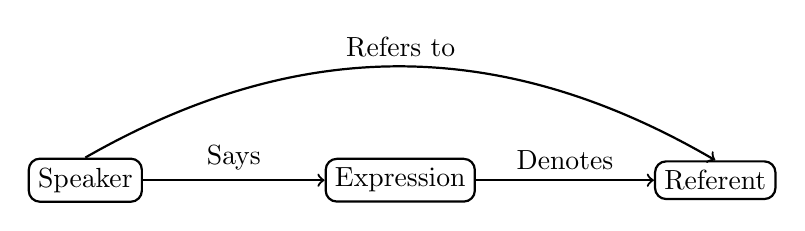
\begin{tikzpicture}[node distance=4cm, auto, thick]
  \node[draw, rounded corners](speaker){Speaker};
  \node[draw, rounded corners, right of=speaker](expression){Expression};
  \node[draw, rounded corners, right of=expression](referent){Referent};

  \draw[->, thick] (speaker) -- node{Says}(expression);
  \draw[->, thick] (expression) -- node{Denotes}(referent);
  \draw[->, thick, bend left] (speaker.north) to node[above]{Refers to}(referent.north);
\end{tikzpicture}
\end{center}


 The \txx{referential view} is focused on direct relationships between
 expressions (words, sentences) and things in the world (realist
 view).

 \end{frame}

\begin{frame}{Representational View}

\begin{center}
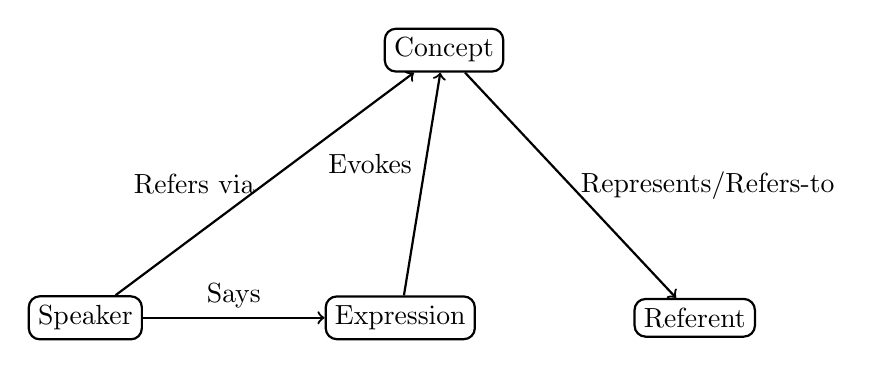
\begin{tikzpicture}[node distance=4cm, auto, thick]
  \node[draw, rounded corners](speaker){Speaker};
  \node[draw, rounded corners, right of=speaker](expression){Expression};
  \node[draw, rounded corners, above right=of expression, xshift=-4cm, yshift=0cm] (concept) {Concept};
  \node[draw, rounded corners, right=of expression, xshift=-2cm] (referent) {Referent};

  \draw[->, thick] (speaker) -- node{Says}(expression);
  \draw[->, thick] (expression) -- node{Evokes}(concept);
  \draw[->, thick] (concept) -- node[right]{Represents/Refers-to}(referent);
  \draw[->, thick] (speaker) to node[left]{Refers via}(concept);
\end{tikzpicture}
\end{center}

 The \txx{representational view} is focused on how relationships between
 expressions (words, sentences) and things in the world are mediated by
 the mind (cognitive linguistics).  

This gives a more complex, but richer model.


\end{frame}

\begin{frame}{Referring vs Non-Referring}

\begin{itemize}
\item \txx{Referring expressions} are expressions that identify
  entities in the world (typically \txx{nominals})
  \begin{exe}
    \ex \eng{cat}, \jpn[that yellow bag]{ano kiiro kaban}
    \ex \eng{London Bridge}, \eng{Xiao Ming}
  \end{exe}
\item \txx{Non-referring expressions} don't have referential properties
  \begin{exe}
    \ex \eng{maybe, if, is, but}
  \end{exe}
\item Not all nominals refer
  \begin{exe}
    \ex \eng{That is \ul{an ugly dog}}
    \ex \eng{If only I had \ul{a dog}}
  \end{exe}
\item And, of course, all this is made more confusing if we model the
  fictional world and our interpretation of it as separate from the
  characters' interpretations, \ldots
\end{itemize}
\end{frame}



\begin{frame}{Further Reading}

\begin{itemize}
\item Introduction What does it mean to mean?
  \begin{itemize}
  \item Saeed: \S~2
  \end{itemize}
\end{itemize}
\end{frame}




%\section{Deixis}

\begin{frame}{What is Deixis}
\begin{itemize}
\item any linguistic element whose interpretation
  necessarily makes reference to properties of the
  extra-linguistic context in which it occurs is \txx{deictic}
  \begin{description}
  \item[\txx{Person}] relative to the speaker and addressee; \eng{you, me, them}
  \item[\txx{Spatial Location}] demonstratives; \eng{this, that, over there, here}
  \item[\txx{Temporal Location}] tense; \eng{yesterday, today, tomorrow}
  \item[\txx{Social Status}] relative to the social position: \eng{professor, you, uncle, boy}
  \end{description}
\item \txx{Discourse deixis}: referring to a linguistic expression or chunk of discourse
\end{itemize}

\newpage
More than 90\% of the declarative sentences people utter are indexical
in that they involve implicit references to the speaker, addressee,
time and/or place of utterance in expressions like first and second
person pronouns, demonstratives, tenses, and adverbs like \lex{here}, \lex{now},
\lex{yesterday} \citep[p366]{Bar-Hillel:1954}.

\end{frame}

\begin{frame}{Spatial Deixis}
\begin{itemize}
\item Two way systems (English, \ldots)
  \\[2ex] \begin{tabular}{llll}
    \txx{proximal} &\lex{this} & \lex{here} &close to the speaker\\
    \txx{distal} &\lex{that} & \lex{there} & far from the speaker 
  \end{tabular}
\item Three (four) way systems (Japanese, \ldots)
    \\[2ex] \begin{tabular}{lllll}
                    & Gloss & \con{thing}   & \con{place}  \\
\hline
      \txx{proximal}  & close to speaker & \lex{kore} ``this'' & \lex{koko} ``here''\\
      \txx{medial} &close to addressee &\lex{sore} ``that''   & \lex{soko} ``there'' \\
      \txx{distal} &far from both&\lex{are} ``\,'tother'' & \lex{asoko} ``over there''  \\ \hline
      \txx{Q} & interrogative & \lex{dore} ``what'' & \lex{doko} ``where''
  \end{tabular}
\end{itemize}
\begin{taskb}
   Can you do English \con{time}? 
\end{taskb}
\begin{taskb}
   Can you do these in another language? 
\end{taskb}
 % Can decompose: \lex{here} ``this place'', \lex{there} ``that place'', \lex{where} ``what place''
 % \lex{now} ``this time'',  \lex{then} ``that time'', \lex{when} ``what time''

 % \noindent\begin{tabular}{lllll}
%     & close to sp  & \multicolumn{2}{c}{far from sp} & Q \\  
%     & & close to hr & far from both \\ \hline
%   English & this & \multicolumn{2}{c}{that} & what \\
%   \ \ \ \  place & here & \multicolumn{2}{c}{there} & where \\
%   Japanese & kono & sono & ano & dono \\
%    \ \ \ \  place & koko & soko & asoko & doko \\
% \end{tabular}


% \mytask{try this}

% \begin{tabular}[l]{}
%   Q & close & far & further \\
%   what & this & that & 'tother \\
%   ?    & now  & then & --- \\
%   where & ? & there & over there \\
% \end{tabular}


\end{frame}

\begin{frame}{More Spatial Deixis}

\begin{itemize}
\item Often lexicalized:
  \begin{itemize}
  \item \lex{go, come, foreign, home, local, indigenous, national language}
  \end{itemize}
\item Can lead to \txx{discourse}/\txx{textual deixis}
  \begin{exe}
    \ex \eng{\ul{Here} we begin explaining textual deixis}
  \end{exe}
\item Often also used for time
  \begin{exe}
    \ex \eng{\ul{This year} we are trying a new kind of assignment}
  \end{exe}
\newpage
\item Spatial expressions extend to possession in many languages
  \begin{exe}
    \ex \gll \jpn{NICT-ga} \jpn{Kyoto-ni} \jpn{aru} \\
    NICT-\textsc{nom} Kyoto-\textsc{loc} be \\
    \trans NICT is in Kyoto
    \ex \gll \jpn{watashi-ni} \jpn{musuko-ga}  \jpn{aru} \\
     I-\textsc{loc}  son-\textsc{nom} be \\
    \trans I have a son (lit. a son is in me)
   \end{exe}
\end{itemize}

\end{frame}

\begin{frame}{Person Deixis}

\begin{itemize}
\item Minimally a three way division
\\[2ex]  \begin{tabular}{lll}
    First Person & Speaker & \lex{I} \\
    Second Person & Addressee & \lex{you} \\
    Third Person & Other & \lex{he/she/it} \\
  \end{tabular}
\item Often combined with
  \begin{itemize}
  \item \txx{gender}: \lex{he/she/it }
  \item \txx{number}: \lex{I/we}, 
    \lex{'anta} ``you:m'', \lex{'antumaa} ``you:dual'',  \lex{'antum} ``you:m:pl''
    \\ (Arabic)
  \item \txx{inclusion}: \lex{n\'uy} ``we including you'',  \lex{n\'{\i}i} ``we excluding you'' (Zayse)
  \item \txx{honorification}: \lex{kimi} ``you:inferior'', \lex{anata} ``you:equal'',
    \\ don't use pronouns for superiors: \lex{sensei} ``teacher'', \ldots (Japanese)
  \end{itemize}
\end{itemize}

\end{frame}

\begin{frame}{Social Deixis}

In European languages, a two-way choice in 2nd person pronominal
reference: the T/V distinction

\begin{itemize}
\item T/V distinctions in European languages
  \\[2ex]
  \begin{tabular}{lll}
    & Familiar 2sg & Polite 2sg \\ \hline
    French & \lex{tu} & \lex{vous} \\
    German & \lex{du} & \lex{Sie} \\
%    Spanish & \lex{t\'u} & \lex{usted} \\
    Czech & \lex{ty} & \lex{vy} \\ 
  \end{tabular}

\item Shift from asymmetric use showing \txx{power} (superior uses \lex{tu}; inferior uses \lex{vous}) to symmetric use showing \txx{solidarity} (strangers use  \lex{vous}; intimates use \lex{tu}): typically the socially superior person must invite the socially
  inferior person to use the familiar form
\end{itemize}

\end{frame}

\begin{frame}{Social Deixis can be marked on other words}
\MyLogo{It must be marked}
\begin{exe}
  \ex \jpn{Tanaka-san-ga kudasaimashita} \hfill [addressee and subject hon.]
  \trans Tanaka gave it to me (and I honor him and you)
%  \trans
 \ex \jpn{Tanaka-san-ga kudasatta} \hfill [subject honorification]
  \trans Tanaka gave it to me (and I honor him)

 \ex \jpn{Tanaka-kun-ga kuremashita} \hfill [addressee honorification]
  \trans Tanaka gave it to me (and I honor you)

 \ex \jpn{Tanaka-kun-ga kureta} \hfill [no honorification]
  \trans Tanaka gave it to me (implies I am higher status than him)

\end{exe}

\begin{taskb}
% \item Find examples where someone addresses Sherlock as \eng{Holmes}
%   and compare then to examples where he is addressed as \eng{Mr
%     Holmes}: what is the difference? \task
Find examples in \textit{Válka s Mloky} or another text where \cs{ty} and \cs{vy} are used:  what is the difference? 
\end{taskb}

\end{frame}

\begin{frame}{Further Reading}
\begin{itemize}
\item Deixis
  \begin{itemize}
  \item Saeed: \S~7.2
  \end{itemize}
\end{itemize}


\end{frame}

\section{Administrivia}



\begin{frame}{Administrivia}
\begin{description}
\item [Coordinator]  Francis \ul{Bond} 
  {\small \url{<bond@ieee.org,francis.bond@upol.cz>}}
\item Course details are all online
\end{description}


\end{frame}

\begin{frame}{Extra Credit}

\begin{itemize}
\item If you submit a correction that gets accepted for one of the
  resources we use then it shows good mastery of the material
  \begin{itemize}
  \item you can get 1-5\% extra credit (depending on the size/difficulty)
\\ Mark $n \propto 10^{n-1}$ lines of code/documentation
  \item You can't go over 100\%
  \end{itemize}
\item A correction can involve
  \begin{itemize}
  \item fixing an error in transcription or annotation
    \begin{itemize}
    \item spelling error
    \item wrong sense
    \item error in the dictionary
    \end{itemize}
  \item making the documentation easy to read
  \item pointing out an error in a translation / finding a new translation
  \item coming up with a good example of a phenomenon
%  \item  fixing a bug in code
%  \item extending the code with new capabilities
  \end{itemize}

\end{itemize}



\end{frame}

\begin{frame}{Student Responsibilities}

By remaining in this class, the student agrees to:
\begin{enumerate}
\item  Make a genuine effort to learn and engage.
\item Read messages and participate.
\item Do assignments on time.
\item Attend regularly.
\item Seek help early, not last minute.
\item Treat peers respectfully.
\end{enumerate}

\end{frame}

\begin{frame}{Attendance}
\begin{enumerate}
\item You are expected to attend all classes.
\item Be on time - lateness is disruptive to your own and others' learning.
\item Valid reasons for missing class include the following:
\begin{enumerate}
\item A medical emergency (including mental health emergencies)
\item A family emergency (death, birth, natural disaster, etc).
\end{enumerate}
\item There will be significant material covered in class that is not in your readings.  You cannot expect to do well without coming to class.
\item If you miss a class, it is your responsibility to get the notes, any handouts you missed, schedule changes, etc. from a classmate.
\end{enumerate}

\end{frame}

\begin{frame}{Remediation and Academic Integrity}
\begin{enumerate}
\item No late work will be accepted, except in the case of a documented excuse.
\item For planned, justified, absences on class days or days on which assignments are due, advance notice must be provided.
\item Cheating will not be tolerated. Violations, including plagiarism, will be seriously dealt with, and could result in \textbf{a failing grade for the entire course}.
\item Refer to the University Honour Code
\item As always, use your common sense and conscience.
\end{enumerate}


\end{frame}


\begin{frame}{The winning strategy}

\begin{itemize}
\item Read the textbook before class (and after again, if necessary)
\item Work together: make study groups
\item Tasks: Discuss as much as you want, annotate your own answers
\item Tutorials: Discuss as much as you want, write your own answers
\item Treat LLMs as though they were a human --- you can discuss the
  answer with them, but they should not give you the entire answer
  
\item Ask questions \ldots\ early and often!
\end{itemize}

\end{frame}









% \begin{frame}[allowframebreaks]
%   \frametitle{References}
%   \bibliographystyle{aclnat}
%   \bibliography{abb,mtg,ling,nlp}
% \end{frame}

\subsection*{Glossary of Key Terms (English--Czech)}

\begin{frame}[allowframebreaks]{Glossary of Key Terms (English--Czech)}
\begin{flushleft}
\begin{longtable}{ll}
  English & Čestina \\\hline \endhead
Q & otázka (Q) \\
analysis & analýza \\
autonomous & autonomní \\
collocation & kolokace \\
communication & komunikace \\
composition & kompozice \\
compositional & kompoziční \\
concordance & konkordance \\
connotation & konotace \\
context & kontext \\
corpus & korpus \\
deictic & deiktický \\
deixis & deixe \\
denotation & denotace \\
discourse & diskurz \\
distal & distální \\
expression & výraz \\
gender &  (gramatický) rod \\
honorification & honorifika \\
idiom & úsloví \\
inclusion & inkluze \\
lexical & lexikální \\
meaning & význam \\
medial & mediální \\
mental lexicon & mentální lexikon \\
metaphor & metafora \\
nominals & nominální výrazy \\
non-referring expressions & nereferenční výrazy \\
number & číslo \\
person & (gramatická) osoba \\
phrase & slovní spojení \\
power & moc \\
pragmatics & pragmatika \\
proximal & proximální \\
refer & odkazovat \\
reference & reference \\
referential & referenční \\
referential view & referenční pohled \\
referring expressions & referenční výrazy \\
representational & reprezentační \\
representational view & reprezentační pohled \\
semantics & sémantika \\
sense & význam (smysl) \\
sentence meaning & význam věty \\
sentiment & sentiment \\
social status & společenský status \\
solidarity & solidarita \\
spatial location & prostorová lokalizace \\
temporal location & časová lokalizace \\
textual deixis & textová deixe \\
utterance & výpověď \\
word meaning (sense) & slovní význam 
\end{longtable}
\end{flushleft}

\end{frame}


\end{document}

%%% Local Variables: 
%%% coding: utf-8
%%% mode: latex
%%% TeX-PDF-mode: t
%%% TeX-engine: xetex
%%% End: 

